\documentclass{beamer}
\usetheme{Bergen}
\usecolortheme{wolverine}

\usepackage{xcolor}
\usepackage{listings}
\usepackage{textcomp}
\usepackage{ulem}
\usepackage{listings}

\title{LLVM at The MathWorks}
\author{Ramkumar Ramachandra}
\institute{The MathWorks}
\titlegraphic{
\includegraphics[scale=0.30]{llvm-matlab}}

\lstset{
  inputencoding=utf8,
  % backgroundcolor=\color{white},
  tabsize=2,
  rulecolor=,
  numbers=none,
  upquote=true,
  % aboveskip={1.5\baselineskip},
  columns=fixed,
  showstringspaces=false,
  extendedchars=true,
  breaklines=true,
  prebreak=\raisebox{0ex}[0ex][0ex]{\ensuremath{\hookleftarrow}},
  frame=single,
  showtabs=false,
  showspaces=false,
  showstringspaces=false,
  basicstyle=\ttfamily\tiny,
  identifierstyle=\ttfamily,
  keywordstyle=[1]\ttfamily\color{blue},
  keywordstyle=[2]\ttfamily\color{purple},
  keywordstyle=[3]\ttfamily\colorbox{yellow},
  commentstyle=\ttfamily\color[rgb]{0.133,0.545,0.133},
  stringstyle=\ttfamily\color[rgb]{0.627,0.126,0.941},
}

\lstdefinelanguage{matlab}{
  morestring=[b]",
  morekeywords=[1]{for, function, zeros, end},
  morekeywords=[2]{},
}

\makeatletter
\lstdefinelanguage{llvm}{
  morecomment = [l]{;},
  morestring=[b]", 
  sensitive = true,
  morekeywords=[1]{
    define, declare, global, constant,
    internal, external, private,
    linkonce, linkonce_odr, weak, weak_odr, appending,
    common, extern_weak,
    thread_local, dllimport, dllexport,
    hidden, protected, default,
    except, deplibs,
    volatile, fastcc, coldcc, cc, ccc,
    x86_stdcallcc, x86_fastcallcc,
    ptx_kernel, ptx_device,
    signext, zeroext, inreg, sret, nounwind, noreturn,
    nocapture, byval, nest, readnone, readonly, noalias, uwtable,
    inlinehint, noinline, alwaysinline, optsize, ssp, sspreq,
    noredzone, noimplicitfloat, naked, alignstack,
    module, asm, align, tail, to,
    addrspace, section, alias, sideeffect, c, gc,
    target, datalayout, triple,
    blockaddress
  },
  morekeywords=[2]{
    add, fadd, sub, fsub, mul, fmul,
    sdiv, udiv, fdiv, srem, urem, frem,
    and, or, xor,
    icmp, fcmp,
    eq, ne, ugt, uge, ult, ule, sgt, sge, slt, sle,
    oeq, ogt, oge, olt, ole, one, ord, ueq, ugt, uge,
    ult, ule, une, uno,
    nuw, nsw, exact, inbounds,
    phi, call, select, shl, lshr, ashr, va_arg,
    trunc, zext, sext,
    fptrunc, fpext, fptoui, fptosi, uitofp, sitofp,
    ptrtoint, inttoptr, bitcast,
    ret, br, indirectbr, switch, invoke, unwind, unreachable,
    malloc, alloca, free, load, store, getelementptr,
    extractelement, insertelement, shufflevector,
    extractvalue, insertvalue,
  },
  morekeywords=[3]{@malloc},
  alsoletter={\%},
  keywordsprefix={\%},
}
\makeatother

\begin{document}
\begin{frame}
  \titlepage
\end{frame}

\begin{frame}{why bother with llvm?}
  \begin{center}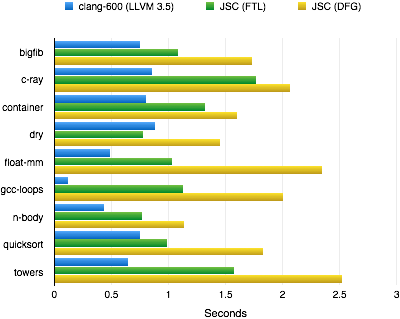
\includegraphics[scale=0.55]{asmjs-ftl-shootout}\end{center}
\end{frame}

\begin{frame}{the hairy C backend}
  \lstinputlisting[language=matlab]{simple_loop.m}
  generates:
  \lstinputlisting[language=c]{simple_loop.c}
\end{frame}

\begin{frame}{the even hairier llvm backend}
  ... [17 pages of crap]
  \lstinputlisting[language=llvm]{hairy.ll}
  ... [does this end?]
\end{frame}

\begin{frame}{let's ask \ttfamily{clang -S -emit-llvm}}
  1 beautiful page
  \lstinputlisting[language=llvm]{clang.ll}
\end{frame}

\begin{frame}{the problem?}
  \begin{itemize}
  \item The LLVM dump is a literal representation of all the data structures in
    memory.
  \item Safety not well thought-out. Inconsistent types come in from frontend,
    and cause crashes.
  \item Maze of different visitors.
  \item Our LLVM usage is basically an in-memory ahead-of-time compile. There is
    no JIT or VM.
  \end{itemize}
  \noindent\rule{8cm}{0.4pt}
  Solution: Possibly introduce a lower intermediate representation of CGIR
  before the final lowering. Start working towards building a VM.
\end{frame}

\begin{frame}{more problems: the fight with upstream}
  \begin{center}
\includegraphics[scale=0.3]{llvm-bug}\end{center}
  \begin{itemize}
  \item MCJIT is buggy on Windows.
  \item MCJIT is slower and uses up more memory than old JIT, if used
    naively.
  \item Many corner case bugs because of Matlab's large memory model.
  \end{itemize}
\end{frame}

\begin{frame}{work that \textit{should} be done}
  \begin{itemize}
  \item A real lazy JIT with object caching.
  \item Different tiers of optimization, triggered with runtime data.
  \item Stackmaps for deoptimization.
  \item Patchpoints for generating the optimized specialized code.
  \end{itemize}
\end{frame}

\begin{frame}{end notes}
  \begin{itemize}
  \item \href{http://blog.llvm.org/2014/07/ftl-webkits-llvm-based-jit.html}{LLVM
      blog: FTL}
  \item
    \href{https://www.webkit.org/blog/3362/introducing-the-webkit-ftl-jit/}{Webkit
      blog: FTL}
  \item
    \href{http://blog.llvm.org/2013/08/object-caching-with-kaleidoscope.html}{LLVM
      blog: object caching}
  \item \href{http://llvm.org/devmtg/2014-10/Slides/Trick-FTL.pdf}{2014 Dev Meet:
      FTL}
  \end{itemize}
\end{frame}

\end{document}
